\chapter{Introducción específica} % Main chapter title

En este capítulo se detallan los componentes y tecnologías que se seleccionaron para utilizar en el trabajo. Además, se van a mencionar los aportes específicos del grupo de estudiantes que colaboró con el inicio del proyecto.

\section{Componentes de hardware}
Para la realización de la capa física hay cuatro componentes indispensables.

\subsection{NodeMCU ESP32}
Este es un microcontrolador que, como se menciona en la web de Espressif, se destaca por sus <<potentes módulos Wi-Fi + Bluetooth/Bluetooth LE que se dirigen a una amplia variedad de aplicaciones AIoT>> [9]. Es importante señalar que en el mundo de ESP existen dos familias, ESP8266 y ESP32. Entre ambas se opta por ESP32 porque es la nueva generación fabricada por Espressif. Además, cuentan con más documentación [10] y poseen mejoras en el hardware. Las cuales están asociadas a una mayor capacidad de procesamiento, de integración y una mejor placa de Wi-Fi. En la hoja de datos de la documentación oficial [11] podemos ver su descripción de hardware. En la figura 2.1, extraída de dicha documentación, podemos ver el diagrama de bloques del ESP32.

\begin{figure}[htpb]
\centering 
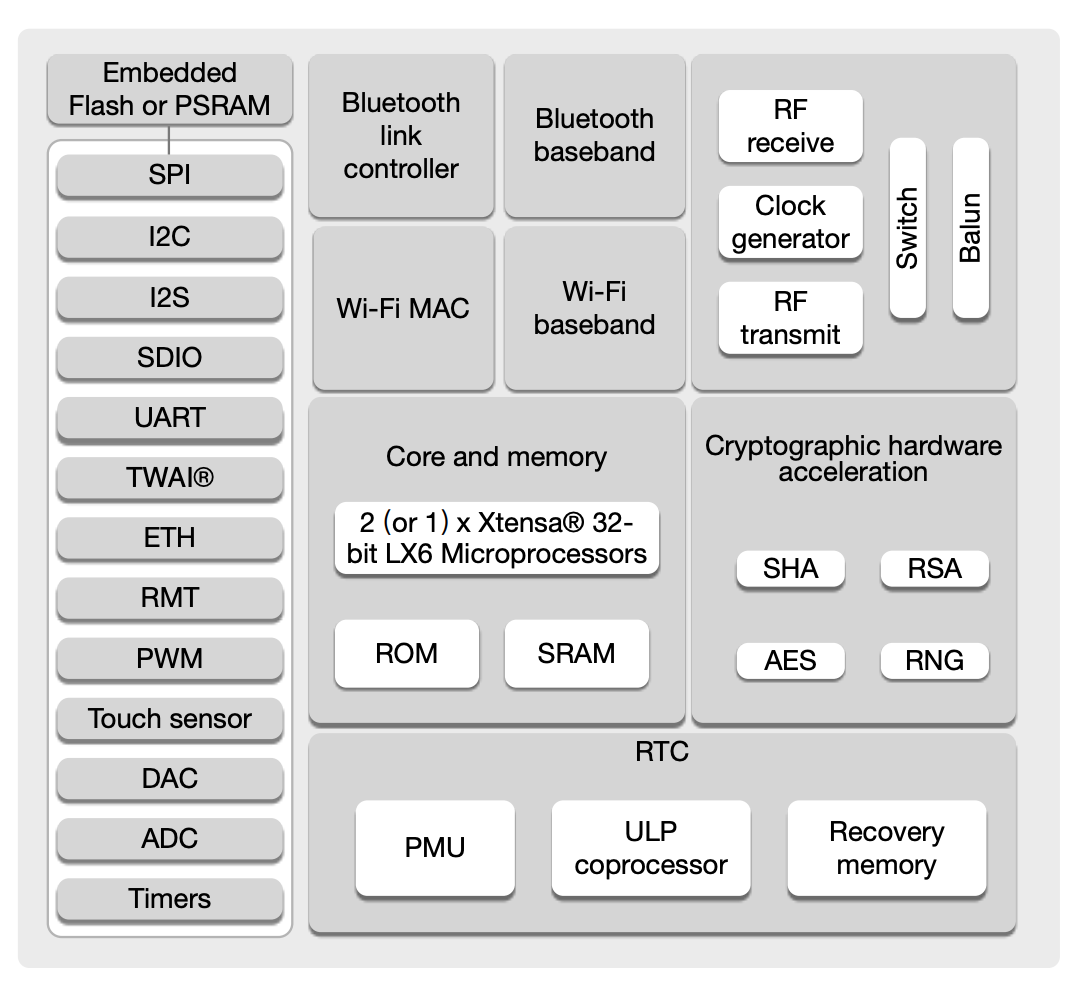
\includegraphics[width=.6\textwidth]{./Figures/esp32hardware.png}
\caption{Diagrama de bloques ESP32.}
\label{fig:diagBloques}
\end{figure}

A su vez, en la familia de ESP32 tenemos diferentes tipos de módulos [12]. Cada uno presenta pequeñas variaciones de hardware, comandos de integración de Firmware y cantidad de pines. En particular, para este trabajo se utiliza el módulo de WROOM. Más específicamente uno de los tableros de ESP32-devkit [13]. Además, existen diferentes versiones de tableros de desarrollo de WROOM para ESP32-DEVKIT. Por ello, para realizar las conexiones con los sensores, es fundamental tener conocimiento sobre la usabilidad de cada uno de los pines de la placa. Aunque esta información está disponible en la hoja de datos oficial, en caso de no tener tanto conocimiento técnico se sugiere revisar le posteo de <<ESP32 Peripherals>> en la web de RandomNerdTutorials [14], ya que es muy útil principiantes en la materia. En la figura 2.2 se presenta un diagrama de pines de dicha web.

\begin{figure}[htpb]
\centering 
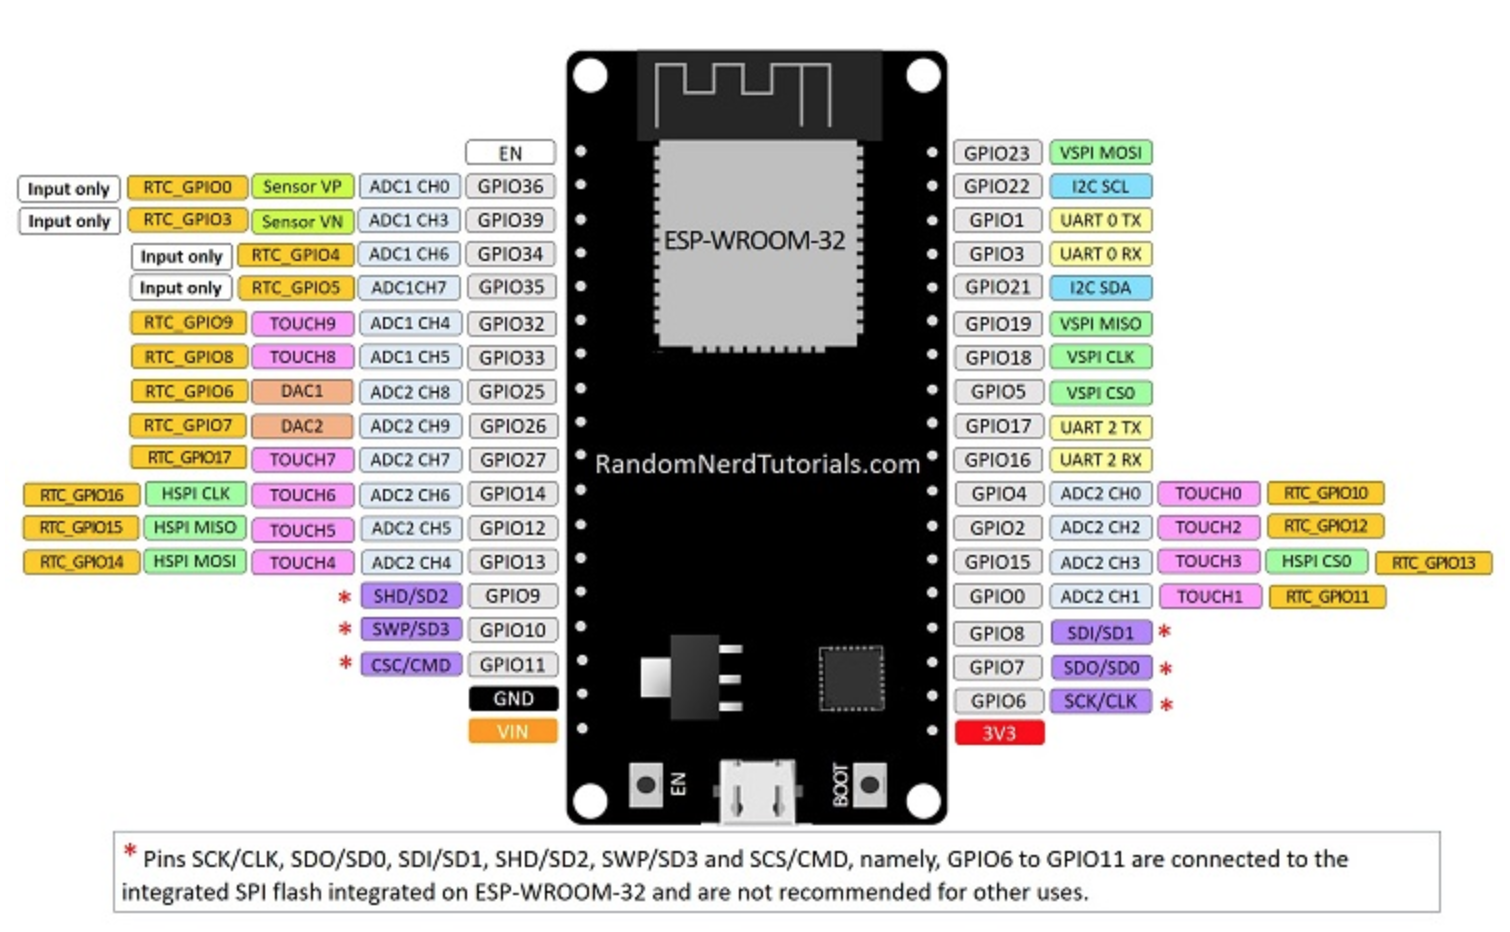
\includegraphics[width=.9\textwidth]{./Figures/esp32pines.png}
\caption{Diagrama pines ESP32.}
\label{fig:diagBloques}
\end{figure}

Para finalizar, se seleccionó esta placa no solo por lo expuesto anteriormente sobre sus bondades en hardware, sino que también, por las que tiene en software. Esto se debe a Espressif ofrece una buena variedad de ejemplos de código C en su repositorio de github [15].

\subsection{Sensor de temperatura y humedad relativa DHT11}
Con este sensor se podrá realizar la obtención de valores de temperatura y humedad ambiente. Según se detalla en su hoja de datos [16] ofrece una señal digital confiable y estable.
Este sensor cuenta con 4 pines, de los cuales usaremos los siguientes 3 (los pines se cuenta de izquierda a derecha con el sensor de frente):
\begin{itemize}
\item Pin 1: VDD (alimentación). Deberá recibir de 3,3 a 6 V. Se recomienda colocar un capacitor de 100nF entre este pin y el pin GND para su protección.
\item Pin 2: DATA. Una vez establecida la conexión, este pin enviará los datos de temperatura y humedad relativa al módulo ESP.
\item Pint 4: GND.
\end{itemize}

\subsection{Sensor de humedad en suelo capacitivo analógico V1.2}
Es un sensor se utiliza para medir la humedad del sustrato. Como se menciona en su hoja de datos [17] es una excelente opción ya que <<está hecho de un material resistente a la corrosión lo que le da una excelente vida útil>>. Cuenta con un conector de pines con las opciones de muy claros, VCC, GND y AOUT (datos analógicos). Se recomienda utilizar con una potencia entre 3,3 a 5 V.

\subsection{ADC ADS1115}
Debido a que el sensor de humedad de suelo tiene mayores pruebas usando arduido (incluso en su hoja de datos) se va a utilizar un convertidor analógico digital con el ESP32. Se utilizaron como fuentes de información su hoja de datos [18] y un tutorial de <<Programar Fácil>>[19] donde se explica su utilidad y usos. De esta forma usaremos la señal analógica del sensor capacitivo para enviar los datos digitales a la placa ESP32.

%----------------------------------------------------------------------------------------

\section{Herramientas de software}

%----------------------------------------------------------------------------------------

\section{Desarrollo UNLa}

%----------------------------------------------------------------------------------------
